\documentclass{ximera}

\graphicspath{{./graphics/}{./content/04_6_substitution/graphics/}}

\title{Optimization with Constraints}
\begin{document}
\begin{abstract}
\end{abstract}
\maketitle

In this section, we will study optimization subject to constraints. For example, suppose we would like the find the maximum value of $f(x,y) = xy$ subject to the constraint $2x+2y=100$. We can think of this as restricting ourselves to the line $2x+2y=100$, and finding the maximum value of $f$ over this line.

\begin{image}
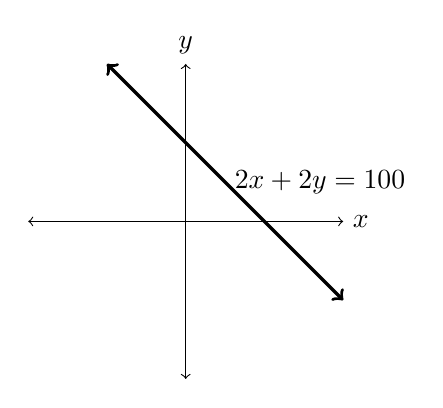
\begin{tikzpicture}
\draw[<->] (-2,0) -- (2,0);
\node[anchor = west] at (2,0) {$x$};
\draw[<->] (0,-2) -- (0,2);
\node[anchor = south] at (0,2) {$y$};

\draw[very thick, <->] (-1,2) -- (2,-1);
\node[anchor = west] at (.5,.5) {$2x+2y=100$};
\end{tikzpicture}
\end{image}

These types of problems often arise in real-world applications: you have some limitation on resources, which provide the constraint, and want to optimize some sort of performance. A classical problem from geometry and single variable calculus is to maximize the area of a rectangle, subject to the constraint that the perimeter is $100m$. Setting up the problem algebraically, this is equivalent to finding the maximum value of $f(x,y) = xy$ subject to the constraint $2x+2y=100$. In single variable calculus, we could solve for $y$ in the second equation, and use this to reduce the objective function, $f(x,y)$, to a single variable function, which we would them optimize. That is, from $y=50-x$, we would have
\begin{align*}
g(x) &= f(x,50-x)\\
&= x(50-x)\\
&= 50x-x^2.
\end{align*}
Differentiating $g$, we get
\[
g'(x) = 50-2x.
\]
So, we have $g'(x) = 0$ when $x = 25$. The second derivative of $g$ is $g''(x) = -2<0$, so $g$ has a local maximum at $x=25$. Since $g$ is continuous on all of $\mathbb{R}$ and has only one critical point, this means that $g$ has an absolute maximum at $x=25$. So, the maximum value of $f$ is
\[
f(25,50-25) = g(25) = 15625.
\]

For optimization subject to a constraint for multivariable functions in general, we'll follow a similar process: use the constraint to make a substitution, and then optimize the resulting function. However, we'll soon see that this can be much more complicated than it was in the single variable case, and it requires paying careful attention to constraints and domains.

\section*{Optimization with Constraints}

Let's consider a higher dimensional version of the problem from the introduction. That is, let's try to find the maximum value of $f(x,y,z) = xyz$ subject to the constraint that $x+y+z=30$. Taking the constraint $x+y+z=30$ and solving for $z$, we have $z = 30-x-y$. Using substitution, we can reduce the function $f$ to a function of two variables,
\begin{align*}
g(x,y) &= f(x,y,30-x-y)\\
&= xy(30-x-y)\\
&= 30xy-x^2y-xy^2.
\end{align*}
So, we'd like to optimize $g$. In order to do this, we'll find the critical points of $g$. For this, we first find the gradient of $g$.
\[
\nabla g(x,y) = (30y-2xy-y^2, 30x-2xy-x^2)
\]
Solving $(30y-2xy-y^2, 30x-2xy-x^2) = (0,0)$, we find two critical points: $(0,0)$ and $(10,10)$. Let's use the Hessian matrix of $g$ to determine the behavior of $g$ at these critical points.
\[
Hg(x,y) = \begin{pmatrix}
-2y & 30-2x-2y\\
30-2x-2y & -2x
\end{pmatrix}
\]
At $(0,0)$, the Hessian matrix is
\[
Hg(x,y) = \begin{pmatrix}
0 & 30\\
30 & 0
\end{pmatrix}.
\]
This corresponds to the quadratic form $p(x,y) = 60xy$, which is indefinite. So, $g$ has a saddle point at $(0,0)$.

At $(10,10)$, the Hessian matrix is
\[
Hg(x,y) = \begin{pmatrix}
-20 & -10\\
-10 & -20
\end{pmatrix}.
\]
Using Sylvester's Theorem, this matrix is negative definite. So, $g$ has a local maximum at $(10,10)$. But does this mean that $g$ has an absolute maximum at $(10,10)$? Let's look at the graph of $g$ to investigate.

\begin{image}
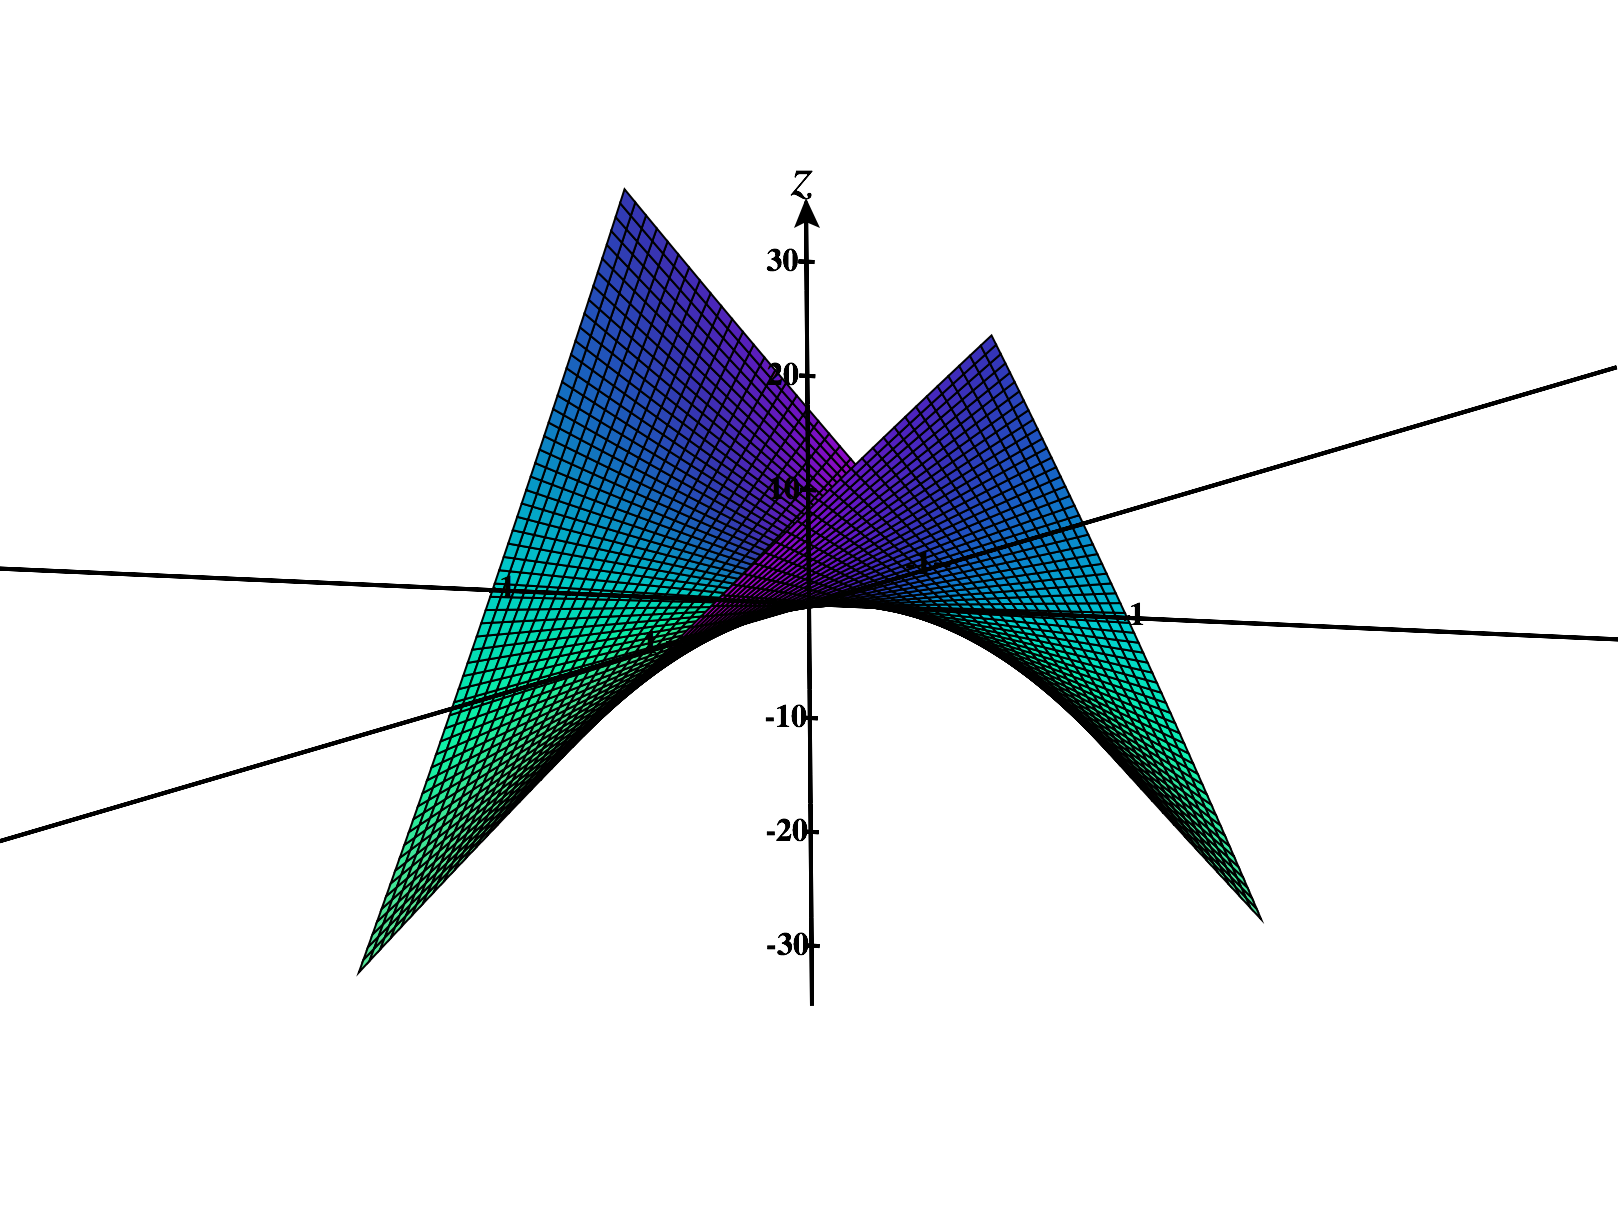
\includegraphics[width = \textwidth]{CalcPlot3D-saddle}
\end{image}

We see that $g$ actually doesn't have any absolute maximum (or minimum) - it's values get arbitrarily large, and arbitrarily small. So, here we see an example where the multivariable situation is more nuanced than the single variable situation. Often, it will be difficult to determine if multivariable functions have absolute extrema using the methods that we've covered so far. However, in the case where we're optimizing a continuous function over a compact region, we know that absolute extrema exist. Because of this fact, we will focus most of our attention on this special situation.

With that in mind, let's consider a revised version of our previous problem.

\begin{example}
We'll find the maximum and minimum values of $f(x,y,z) = xyz$ subject to the constraints that $x+y+z=30$, and $x$, $y$, and $z$ must be \emph{nonnegative}.

If we consider the set of $(x,y,z)$ such that $x+y+z=30$, and $x,y,z\geq 0$, we see that this is a triangle in $\mathbb{R}^3$, and that it is a compact region. Since $f$ is a continuous function, the Extreme Value Theorem guarantees that it will achieve and absolute maximum and minimum. We could optimize this function using our earlier methods for compact regions, but we'll instead optimize using substitution.

Substituting $z = 30-x-y$, we reduce $f$ to a function of two variables,
\begin{align*}
g(x,y) &= f(x,y,30-x-y)\\
&= xy(30-x-y)\\
&= 30xy-x^2y-xy^2.
\end{align*}
Keeping our previous constraints in mind, we want to optimize $g$ over the region $X = \{(x,y)\;:\;x\geq 0, y\geq 0, \text{ and } 30-x-y\geq 0\}$. Graphing this region in $\mathbb{R}^2$, we see that $X$ is a compact region, hence $g$ has an absolute maximum and absolute minimum over $X$.

\begin{image}
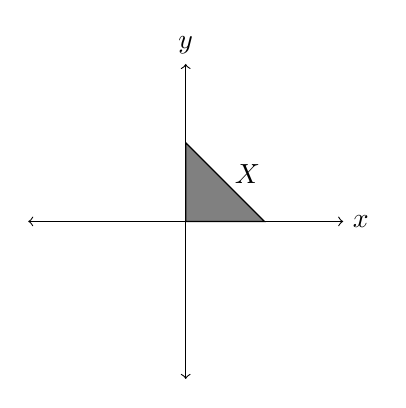
\begin{tikzpicture}
\draw[<->] (-2,0) -- (2,0);
\node[anchor = west] at (2,0) {$x$};
\draw[<->] (0,-2) -- (0,2);
\node[anchor = south] at (0,2) {$y$};

\draw[fill = gray] (0,0) --(1,0) -- (0,1) -- (0,0);
\node[anchor = west] at (.5,.6) {$X$};
\end{tikzpicture}
\end{image}

We find the gradient of $g$ to find the critical points in $X$,
\[
\nabla g(x,y) = (30y-2xy-y^2, 30x-2xy-x^2),
\]
and solving $(30y-2xy-y^2, 30x-2xy-x^2) = (0,0)$, we find two critical points: $(0,0)$ and $(10,10)$. Evaluating $g$ at these critical points, we find
\begin{align*}
g(0,0) &= 0,\\
g(10,10) &= 1000.
\end{align*}
Now, let's examine $g$ on the boundary of $X$. The boundary of $X$ consists of three line segments, along which we have $x = 0$, $y=0$, or $30-x-y=0$. In each of these cases, $g(x,y) = 0$, so $g$ is zero along the entire boundary of $X$.

Comparing the values that we've found, we see that $g$ has an absolute maximum of $1000$ at $(10,10)$, and an absolute minimum of $0$ which occurs along the line segments $x=0$, $y=0$, and $30-x-y=0$.

Translating this back to our original function $f$, the absolute maximum of $f$ subject to the constraint $x+y+z=30$ for nonnegative $x,y,z$ is $1000$, which occurs at the point $(10,10,10)$. The absolute minimum is $0$, which occurs when $x=0$, $y=0$, or $z=0$.

\end{example}

We'll now look at another example where optimizing a multivariable function subject to a constraint using substitution is deceptively difficult.

\begin{example}
We'll find the absolute maximum and absolute minimum of $f(x,y) = x^2-y^2$ subject to the constraint $x^2+y^2=1$.

\begin{image}
\begin{tikzpicture}
\draw[<->] (-2,0) -- (2,0);
\node[anchor = west] at (2,0) {$x$};
\draw[<->] (0,-2) -- (0,2);
\node[anchor = south] at (0,2) {$y$};

\draw (0,0) circle (1);
\node[anchor = west] at (.8,.8) {$x^2+y^2=1$};
\end{tikzpicture}
\end{image}

Since $\{(x,y)\;:\;x^2+y^2=1\}$ is a compact region, and $f$ is a continuous function, the Extreme Value Theorem tells us that $f$ will have an absolute maximum and minimum.

Let's rewrite the constraint as $x^2=1-y^2$, and substitute this into $f$ to reduce $f$ to a function of a single variable:
\begin{align*}
g(y) &= (1-y^2)-y^2\\
&= 1-2y^2.
\end{align*}
Differentiating $g$, we obtain
\[
g'(y) = -4y.
\]
This has one critical point, $y=0$. Taking the second derivative of $g$, we have
\[
g''(y) = -4,
\] 
so $g$ has a local maximum at $y=0$. Since $g$ only has one critical point and it's a local maximum, $g$ has an absolute maximum at $y=0$. Furthermore, $g$ has no absolute minimum.

However, we said that $f$ must have an absolute minimum, so something must be wrong! Here, we've lost track of some of the information contained in our constraint. Consider again
\[
x^2= 1-y^2.
\]
Since $x^2\geq 0$ for all $x$, we must have $-1\leq y\leq 1$. So, we should really be optimizing $g$ over the closed interval $[-1,1]$. We've already found the critical point, $y=0$, of $g$. Comparing the value of $g$ at this points and the endpoints of the interval, we have
\begin{align*}
g(0) &= 1,\\
g(-1) &=-1,\\
g(1) &= -1.
\end{align*}
So, we see that $g$ has an absolute maximum of $1$ at $y=0$, and an absolute minimum of $-1$ at $y=-1$ and $y=1$.

Translating this back to our original function, $f$ has an absolute maximum of $1$ at $(\pm 1, 0)$, and an absolute minimum of $-1$ at $(0,\pm 1)$.

We can see this reflected in the graph of $f$ over $x^2+y^2=1$; the edge of the saddle shape graphed below.

\begin{image}
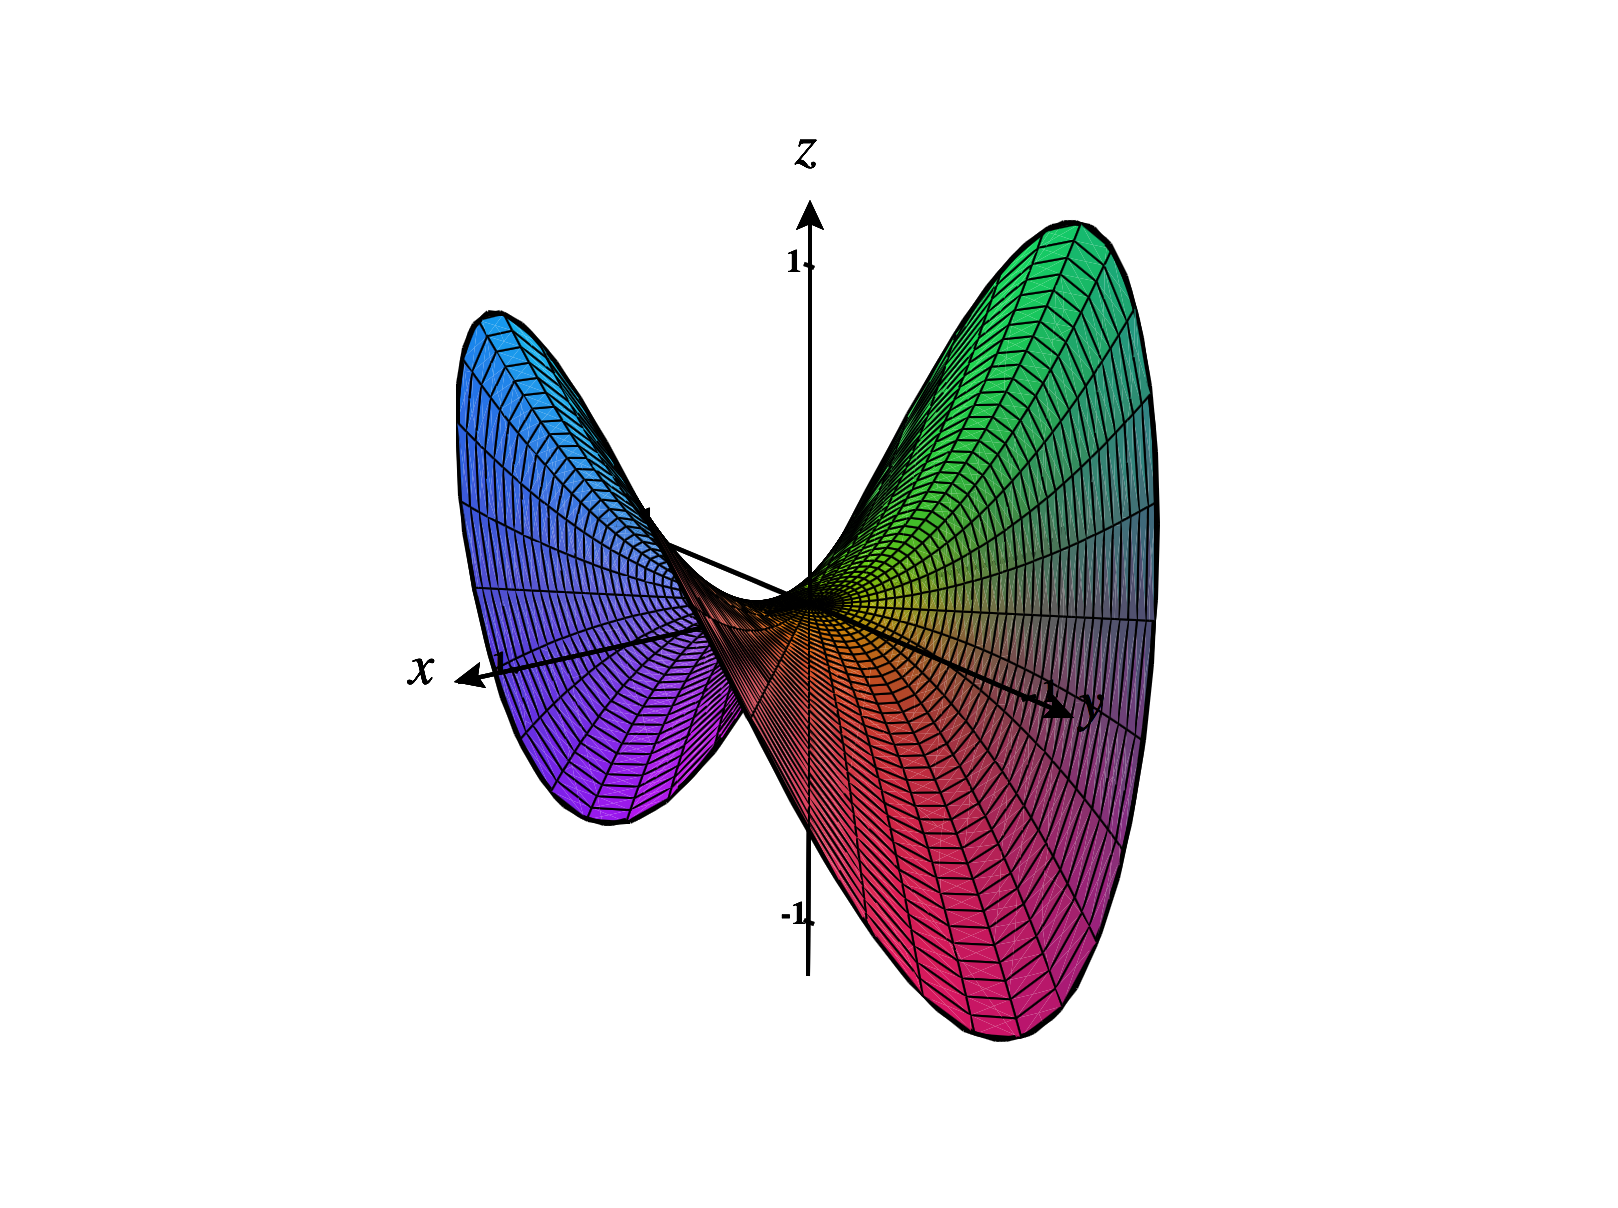
\includegraphics[width=\textwidth]{CalcPlot3D-pringle}
\end{image}

\end{example}

The moral of this section is: weird things can happen with multivariable functions, and you need to be very careful with constraints.

\end{document}